
\begin{figure}
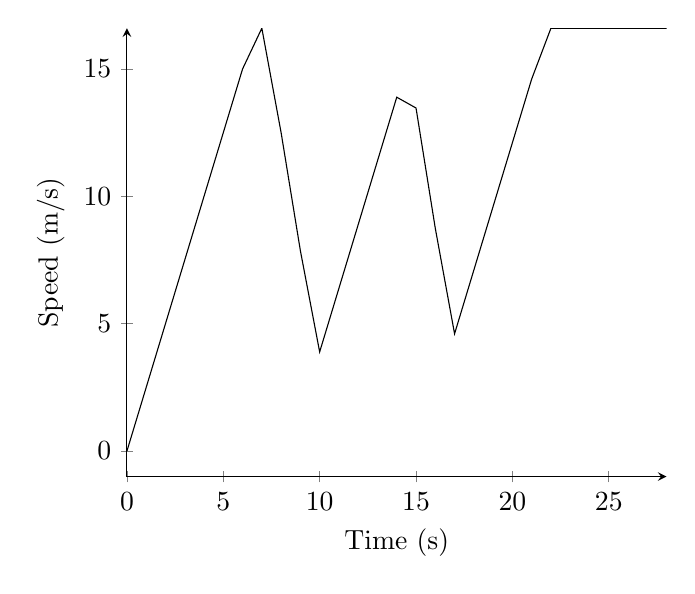
\begin{tikzpicture}
\begin{axis}[
legend style={
	anchor=west
},
axis x line=bottom,
axis y line=left,
ymin=-1,
point meta=explicit symbolic,
xlabel=Time (s),
ylabel=Speed (m/s)
]
\addplot[] coordinates {
(0, 0.0)
(1, 2.5)
(2, 5.0)
(3, 7.5)
(4, 10.0)
(5, 12.5)
(6, 15.0)
(7, 16.6)
(8, 12.4997297278)
(9, 7.8651809677)
(10, 3.8924755069)
(11, 6.3924755069)
(12, 8.8924755069)
(13, 11.3924755069)
(14, 13.8924755069)
(15, 13.4677307676)
(16, 8.74380453035)
(17, 4.60443858321)
(18, 7.10443858321)
(19, 9.60443858321)
(20, 12.1044385832)
(21, 14.6044385832)
(22, 16.6)
(23, 16.6)
(24, 16.6)
(25, 16.6)
(26, 16.6)
(27, 16.6)
(28, 16.6)
};

\end{axis}
\end{tikzpicture}
\label{tik:50:14_V, 13_N, 13_N.-40, 12_V}
\caption{50 percent diving with GSC on route $14_V, 13_N, 13_N.-40, 12_V$}
\end{figure}
